%%%%%%%%%%%%%%%%%%%%%%%%%%%%%%%%%%%%%%%%%%%%%%%%%%%%%%%%%%%%%%%%%%%%%%%%
%                                                                      %
%     File: Thesis_Bootrom.tex                        %
%     Tex Master: Thesis.tex                                %
%                                                                      %
%     Author: Carlos A. Rodrigues                         %
%     Last modified : 15 Abril 2013                         %
%                                                                      %
%%%%%%%%%%%%%%%%%%%%%%%%%%%%%%%%%%%%%%%%%%%%%%%%%%%%%%%%%%%%%%%%%%%%%%%

\chapter{Testes de funcionamento}
\label{chapter:teste}

No desenvolvimento do sistema onde existem vários Cores que podem se ligar e desligar facilmente do sistema, podendo ser complexo manter uma versão estável com tantos cores disponiveis e em desenvolvimento ao mesmo tempo. Percebeu-se que seria bastante interessante o desenvolvimento de um sistema de testes para os sistema, escolheu-se integrar o sistemas ao "fusesoc" para tornar um processo simples de correr e ainda é utilizado apenas uma ferreamente para todo o que precisa de se fazer (melhor isto). Este sistema de testes tinha de permitir desenvolver facilmente testes para os vários cores existentes, também que permita correr os testes nos vários sistemas ou seja na placa de FPGA ou mesmo num simulador do sistema em Verilator, para alem destas duas funcionalidades que permita efectuar apenas o teste a um único cores, ou efectuar uma bateria de teste a todos os cores que tenham teste desenvolvido.

Com as especidades anterior-se percebes-se que seria enevitavel existir imformação a espscificar o teste de cada core. Para isso todos os testes de core têm especificamente um pasta com o nome do core que vai testar, dentro de cada pasta o teste é constituido por um ficheiro em python com o nome test.py, um ficheiro Makefile e por fim um ficheiro com um programa escrito em C com o nome do teste ponto C, por exemplo se for o teste da Rom a pasta vai-se chamar Rom e o ficheiro com o programa em C seria Rom.C. O ficheiro python é constituido por tres metodos com os nomes verilator, icarus e board, cada metodo corresponde ao processo de preparação, execução e verificação do teste para cada plataforma. Por exemplo o metodo com o nome verilator compila o programa que vai carregar no sistema em modo de simulador, criar os meios necessarios para comunicação com o sistema em simulação, executa o processo de simulação e por fim com a resposta do sistema verifica se o core está a funcionar correctamente. No ficheiro Makefile existem 3 "não sei o nome" sim, board e clean. O clean como o nome indica apaga todos os ficheiros criados no processo de execução do teste. No caso do sim e board correspondem a compilação do ficheiro escrito em na linguagem C, um para a execução no simulador e outro para ser executado na placa FPGA, respectivamente. O ficheiro com o programa em C corresponde a uma programa simples, para ser o mais rápido possível, que teste o core pretendido.

O maior problema nos desenvolvimentos dos testes era como obter o resultado pelo computador para ficar registado e apresentado ao utilizador. A solução encontrada foi enviar o resultado a partir do modelo de UART, mas para isso tem de ser testado antes de testar qualquer teste. Uma vez que podemos não receber a mensagem correcta e o problema não ser do core que estamos a testar mas sim do core de UART. O processo de teste é todo efectuado pelo o programa de teste e envia uma determinada mensagem caso este esteja a funcionar correctamente, caso contrario envia uma outra mensagem a informar que não está a funcionar correctamente.

 
explicar as ligações
como foi implementado no Orpsoc. 

adicionar uma imagem explicativa como foi implementado.
\begin{figure}[!htb]
  \centering
  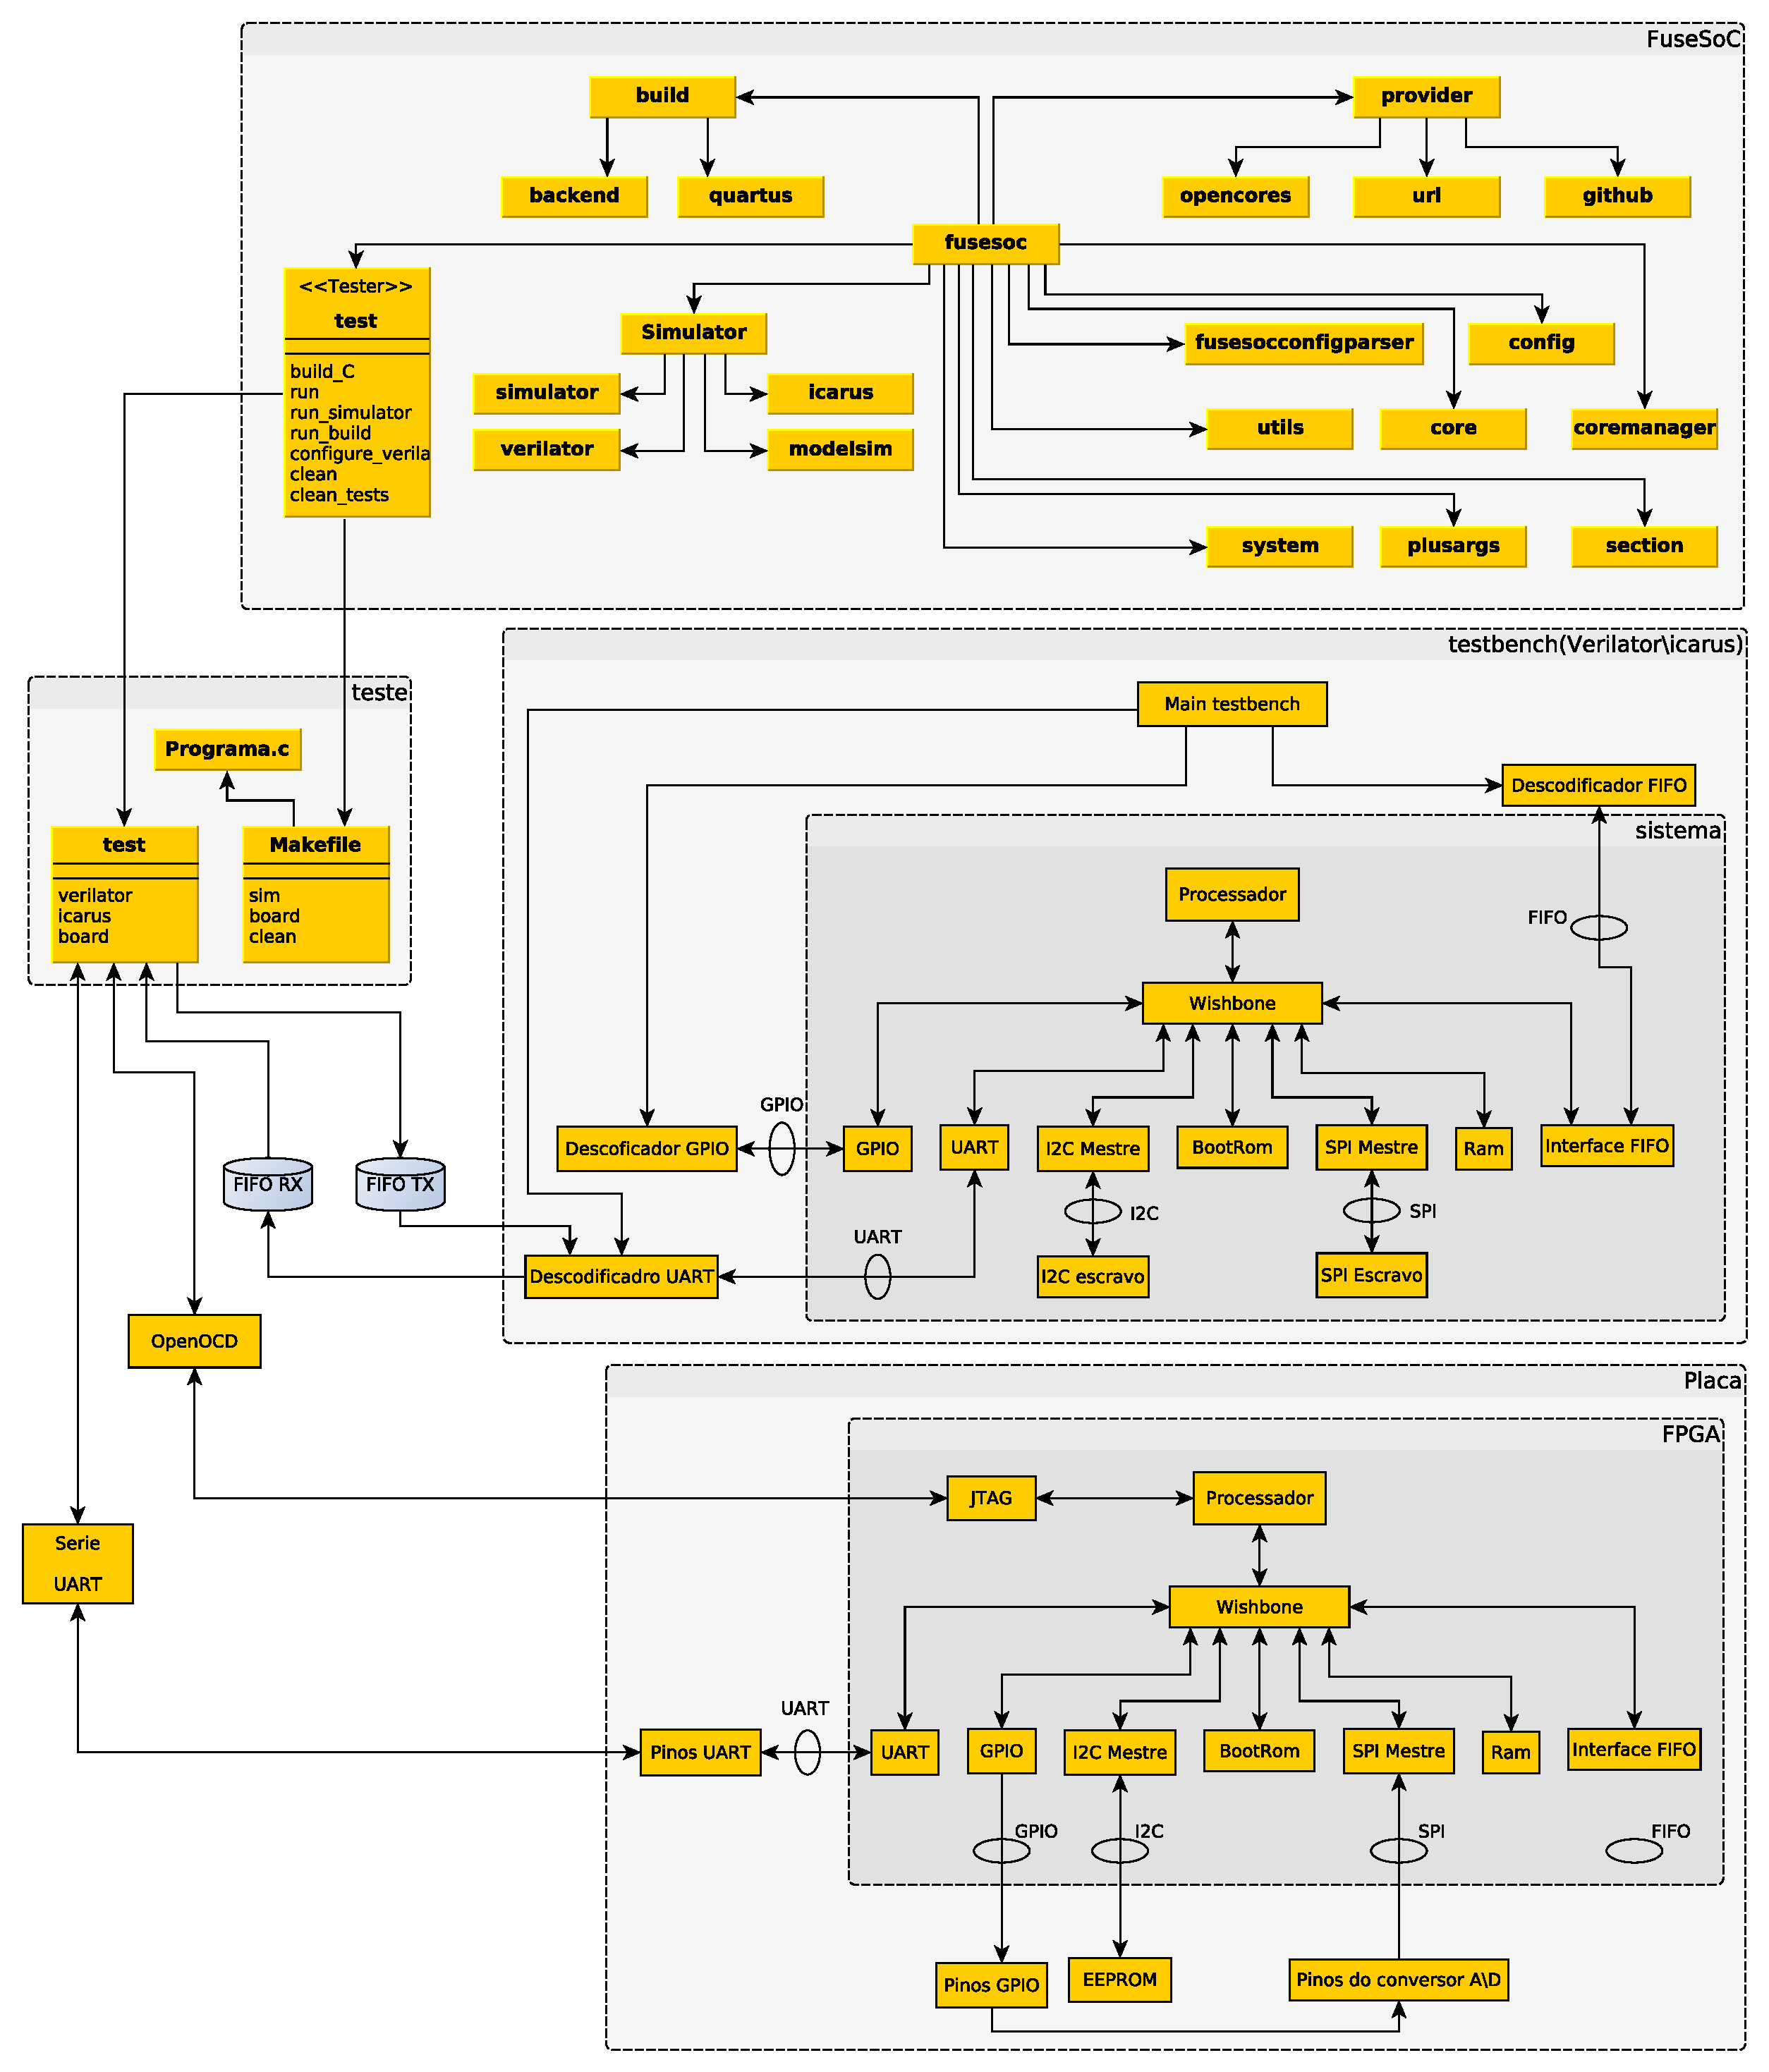
\includegraphics[width=1.00\textwidth]{grafos/Fusesoc_teste.pdf}
  \caption[Diagrama de da plataforma de testes usando o Fusesoc]{Diagrama da plataforma de testes usando o Fusesoc.}
  \label{fig:fusesoc_teste}
\end{figure}


falar sobre as flags do teste
\begin{table}[h!]
  \begin{center}
    \begin{tabular}{|c|C{8cm}|c|}
      \hline
      parametro & Descrição & Default \\
      \hline \hline
      --test & Corre apenas o teste indicado & Corre todos os testes existentes na pasta. \\
      \hline
      --mode & Indica com que ferramenta se pretende fazer os testes  (verilator,icarus,board). & Corre os teste com o verilator. \\ 
      \hline
      --folder & Selectionar uma pasta alternativa com os testes, a partir da raiz. & Selectiona a pasta './orpsoc/orpsoc/test/'.\\
      \hline
      system & Selecionar qual dos sistemas se pretende testar. & Parametro obrigatorio.\\
      \hline
    \end{tabular}
  \end{center}
  \caption[Tabela com os parametros existentes na função de correr testes]{Tabela com os parametros existentes na função de correr testes}
  \label{table:Flags}
\end{table}

como posso ver os resultados dos teste

\section{adicionar novos testes}

fazer novos testes.

\section{Testes desenvolvidos}

para mostrar que o sistema funciona corremante foi desenvolvido estes testes 

\subsection{SPI}

explicar como é testado

\subsubsection{simulador verilator}

\subsubsection{Board FPGA}

\subsection{I2C}

explicar como é testado

\subsubsection{simulador verilator}

\subsubsection{Board FPGA}

\subsection{Interface FIFO}

explicar como é testado

\subsubsection{simulador verilator}

\subsubsection{Board FPGA}

\subsection{Bootrom}

explicar como é testado

\subsubsection{simulador verilator}

\subsubsection{Board FPGA}
